\documentclass[border=10pt,tikz]{standalone}
\usepackage{tikz}
\usepackage{xcolor}
\usepackage[T1]{fontenc}
\usepackage{lmodern}
\usetikzlibrary{positioning,arrows.meta,decorations.pathreplacing,decorations.markings,calc,fadings,patterns}

\definecolor{ink}{HTML}{0E1116}
\definecolor{inksoft}{HTML}{3A3F47}
\definecolor{inkmute}{HTML}{6A7079}
\definecolor{textc}{HTML}{2563EB}
\definecolor{audioc}{HTML}{EA580C}
\definecolor{accentc}{HTML}{7C3AED}
\definecolor{audiogreen}{HTML}{059669}
\definecolor{linec}{HTML}{CFC9B8}
\definecolor{soft}{HTML}{F3F1EA}
\definecolor{warn}{HTML}{B91C1C}

\begin{document}
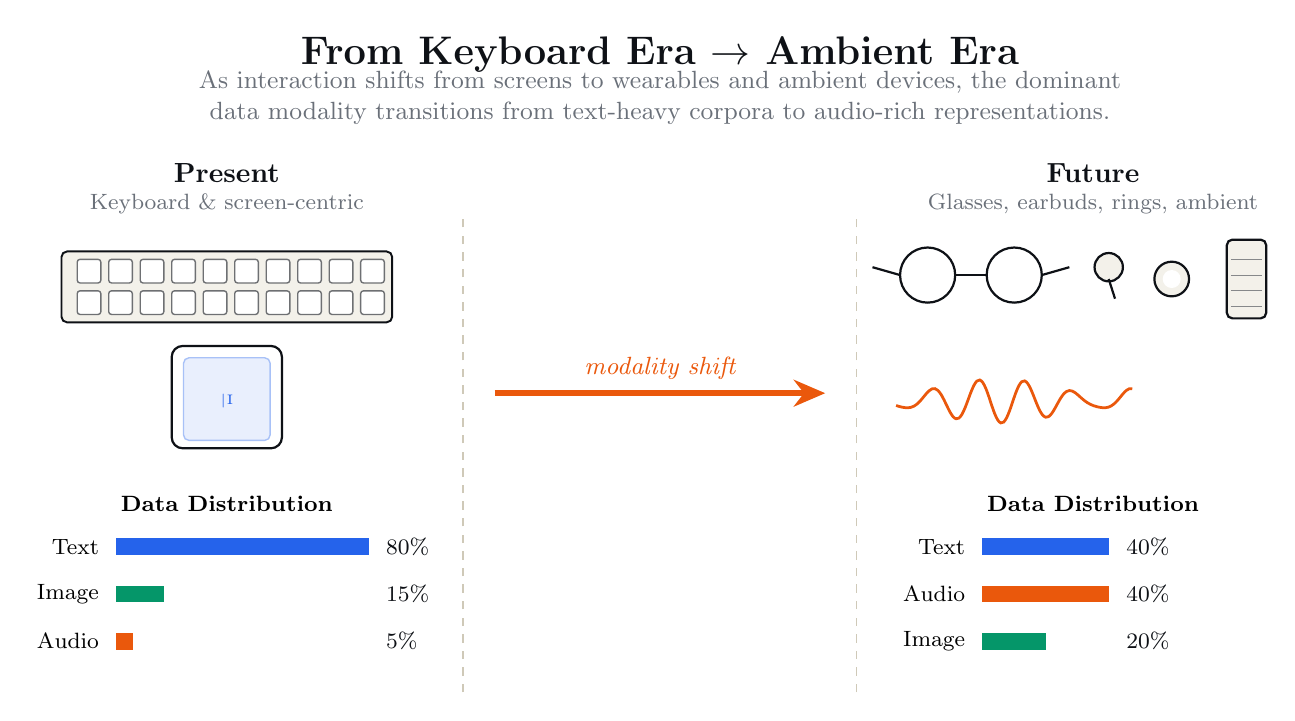
\begin{tikzpicture}[
  font=\sffamily,
  every node/.style={font=\sffamily}
]

% Title
\node[font=\Large\bfseries, color=ink] at (0,5.4) {From Keyboard Era \(\to\) Ambient Era};
\node[font=\small, color=inkmute, text width=14cm, align=center] at (0,4.85) {As interaction shifts from screens to wearables and ambient devices, the dominant data modality transitions from text-heavy corpora to audio-rich representations.};

% LEFT: Present
\node[font=\bfseries, color=ink] at (-5.5,3.9) {Present};
\node[font=\footnotesize, color=inkmute] at (-5.5,3.5) {Keyboard \& screen-centric};

% Keyboard symbol
\draw[rounded corners=2pt, draw=ink, fill=soft, line width=0.7pt] (-7.6,2.0) rectangle (-3.4,2.9);
\foreach \x in {-7.4,-7.0,-6.6,-6.2,-5.8,-5.4,-5.0,-4.6,-4.2,-3.8} {
  \draw[rounded corners=1pt, draw=ink!60, fill=white, line width=0.5pt] (\x,2.1) rectangle ($(\x,2.1)+(0.3,0.3)$);
  \draw[rounded corners=1pt, draw=ink!60, fill=white, line width=0.5pt] (\x,2.5) rectangle ($(\x,2.5)+(0.3,0.3)$);
}

% Phone outline
\draw[rounded corners=4pt, draw=ink, fill=white, line width=0.8pt] (-6.2,0.4) rectangle (-4.8,1.7);
\draw[rounded corners=2pt, draw=textc!40, fill=textc!10, line width=0.5pt] (-6.05,0.5) rectangle (-4.95,1.55);
\node[font=\tiny, color=textc] at (-5.5,1.0) {\textbar I};

% Distribution bars (Present)
\node[font=\footnotesize\bfseries] at (-5.5,-0.3) {Data Distribution};
% Text 80%
\node[font=\footnotesize, anchor=east] at (-7.0,-0.85) {Text};
\draw[fill=textc, draw=textc] (-6.9,-0.95) rectangle (-3.7,-0.75);
\node[font=\footnotesize, color=ink, anchor=west] at (-3.6,-0.85) {80\%};
% Image 15%
\node[font=\footnotesize, anchor=east] at (-7.0,-1.45) {Image};
\draw[fill=audiogreen, draw=audiogreen] (-6.9,-1.55) rectangle (-6.3,-1.35);
\node[font=\footnotesize, color=ink, anchor=west] at (-3.6,-1.45) {15\%};
% Audio 5%
\node[font=\footnotesize, anchor=east] at (-7.0,-2.05) {Audio};
\draw[fill=audioc, draw=audioc] (-6.9,-2.15) rectangle (-6.7,-1.95);
\node[font=\footnotesize, color=ink, anchor=west] at (-3.6,-2.05) {5\%};

% ARROW between
\draw[->, >={Stealth[length=4mm,width=3.4mm]}, line width=2pt, draw=audioc] (-2.1,1.1) -- (2.1,1.1);
\node[font=\small\itshape, color=audioc, anchor=south] at (0,1.15) {modality shift};

% RIGHT: Future
\node[font=\bfseries, color=ink] at (5.5,3.9) {Future};
\node[font=\footnotesize, color=inkmute] at (5.5,3.5) {Glasses, earbuds, rings, ambient};

% Glasses
\draw[draw=ink, line width=0.8pt, fill=white] (3.4,2.6) circle (0.35);
\draw[draw=ink, line width=0.8pt, fill=white] (4.5,2.6) circle (0.35);
\draw[draw=ink, line width=0.8pt] (3.75,2.6) -- (4.15,2.6);
\draw[draw=ink, line width=0.8pt] (3.05,2.6) -- (2.7,2.7);
\draw[draw=ink, line width=0.8pt] (4.85,2.6) -- (5.2,2.7);

% Earbud
\draw[draw=ink, line width=0.8pt, fill=soft] (5.7,2.7) circle (0.18);
\draw[draw=ink, line width=0.8pt] (5.7,2.55) -- (5.78,2.3);

% Ring
\draw[draw=ink, line width=0.8pt, fill=soft] (6.5,2.55) circle (0.22);
\draw[draw=white, line width=0.8pt, fill=white] (6.5,2.55) circle (0.10);

% Smart speaker
\draw[draw=ink, fill=soft, line width=0.8pt, rounded corners=2pt] (7.2,2.05) rectangle (7.7,3.05);
\foreach \y in {2.2,2.4,2.6,2.8} {
  \draw[draw=ink!50, line width=0.4pt] (7.25,\y) -- (7.65,\y);
}

% Mic / waveform
\begin{scope}[shift={(4.5,1.0)}]
  \draw[draw=audioc, line width=1pt] plot[domain=-1.5:1.5, samples=80, smooth] (\x, {0.18*sin(360*\x*1.6) + 0.10*sin(720*\x + 30)});
\end{scope}

% Distribution bars (Future)
\node[font=\footnotesize\bfseries] at (5.5,-0.3) {Data Distribution};
% Text 40%
\node[font=\footnotesize, anchor=east] at (4.0,-0.85) {Text};
\draw[fill=textc, draw=textc] (4.1,-0.95) rectangle (5.7,-0.75);
\node[font=\footnotesize, color=ink, anchor=west] at (5.8,-0.85) {40\%};
% Audio 40%
\node[font=\footnotesize, anchor=east] at (4.0,-1.45) {Audio};
\draw[fill=audioc, draw=audioc] (4.1,-1.55) rectangle (5.7,-1.35);
\node[font=\footnotesize, color=ink, anchor=west] at (5.8,-1.45) {40\%};
% Image 20%
\node[font=\footnotesize, anchor=east] at (4.0,-2.05) {Image};
\draw[fill=audiogreen, draw=audiogreen] (4.1,-2.15) rectangle (4.9,-1.95);
\node[font=\footnotesize, color=ink, anchor=west] at (5.8,-2.05) {20\%};

% Subtle background dividers
\draw[draw=linec, line width=0.5pt, dashed] (-2.5,-2.7) -- (-2.5,3.4);
\draw[draw=linec, line width=0.5pt, dashed] (2.5,-2.7) -- (2.5,3.4);

\end{tikzpicture}
\end{document}
